\documentclass[12pt,letterpaper]{article}

\RequirePackage{xcolor}
\definecolor{tecAzul}{cmyk}{1,0.91,0.33,0.25} % según manual de imagen 2016
\definecolor{tecRojo}{cmyk}{0,0.9,0.86,0}     % según manual de imagen 2016

\renewcommand{\familydefault}{\sfdefault}
\usepackage{amsmath} % for the equation* environment
\usepackage{mwe}
\usepackage{graphicx}
\usepackage[spanish]{babel}
\usepackage{multirow}
\usepackage{titlesec}
\titleformat*{\section}%
{\normalfont\Large\bfseries\color{tecAzul}}
\titleformat*{\subsection}%
{\normalfont\large\bfseries\color{tecAzul}}


\usepackage[tmargin=2cm,bmargin=2cm,lmargin=2.5cm,rmargin=2.5cm]{geometry}
\usepackage{textpos}
\usepackage{tikz}
\usepackage{pgfplots}
\usepackage{pgf}

\usepackage[margin=1cm]{caption}

\usepackage{hyperref}

%
% paragraph layout
%
\parindent0em                           % indentation width of first line
\parskip1.3ex                           % space between paragraphs


\newcommand{\EstudianteA}{David F. Duarte Sánchez}

\pgfplotsset{compat=1.17}



\usepackage{listings}
\usepackage{xcolor}

\definecolor{codegreen}{rgb}{0,0.6,0}
\definecolor{codegray}{rgb}{0.5,0.5,0.5}
\definecolor{codepurple}{rgb}{0.58,0,0.82}
\definecolor{backcolour}{rgb}{0.95,0.95,0.92}

\lstdefinestyle{mystyle}{
    backgroundcolor=\color{backcolour},   
    commentstyle=\color{codegreen},
    keywordstyle=\color{magenta},
    numberstyle=\tiny\color{codegray},
    stringstyle=\color{codepurple},
    basicstyle=\ttfamily\footnotesize,
    breakatwhitespace=false,         
    breaklines=true,                 
    captionpos=b,                    
    keepspaces=true,                 
    numbers=left,                    
    numbersep=5pt,                  
    showspaces=false,                
    showstringspaces=false,
    showtabs=false,                  
    tabsize=2
}

\lstset{style=mystyle}



\begin{document}
	
\graphicspath{{./}{./fig/}}

%-------------------------- Title section -------------------------------------%

%
\begin{textblock}{10}[0,0](-0.5,0)
	\large Escuela de Ingeniería Electrónica \\ 
	EL5617 Trabajo Final de Graduación \\
\end{textblock}

%
\begin{textblock}{10}[0,0](2.6,-0.35)
	\begin{flushright}
		
\includegraphics[scale=0.8]{Firma_TEC-4.pdf}
	\end{flushright}
\end{textblock}

%% Title %%
\begin{center}
	\vspace{70mm}
	{\large\color{tecRojo} Trabajo Final de Graduación}
	\par\vspace{8mm}
	{\Large\bf\color{tecAzul}{Bitácora de Trabajo - Entrega 1}}
	\par\vspace{100mm}
	{{\EstudianteA \\ II Semestre 2024} 
	\vspace{8mm}}
\end{center}

\newpage
%------------------------------------------------------------------------------%

\renewcommand{\baselinestretch}{1.1}    % line spacing

%------------------------------------------------------------------------------%

\section{Semana 5}
\subsection{Corrección de anteproyecto}

\bf{Fecha de trabajo:} 29/07/2024.\\
\bf{Objetivo:} Corrección de observaciones realizadas al anteproyecto.

% Please add the following required packages to your document preamble:
% \usepackage{graphicx}
\begin{table}[h!]
    \label{tab:my-table}
    \resizebox{\textwidth}{!}{%
    \begin{tabular}{|l|}
    \hline
    \hline
    \multicolumn{1}{|c|}{Reporte de   actividades} \\ \hline
    \hline
    - Se comienza a realizar una reestructuración de las secciones del anteproyecto, ya que en la lectura \\ 
    de los párrafos se perdía la noción de lo que se deseaba transmitir al lector. Se habla con el      \\ 
    profesor asesor y el mismo recomienda realizar mapas conceptuales con el objetivo de         \\ 
    llevar un mejor orden de ideas.                \\ \hline\hline
    \multicolumn{1}{|c|}{Productos obtenidos}                            \\ \hline\hline
    Se realizaron los mapas conceptuales  que se pueden observar en las Figuras \ref{fig:Entorno} y \ref{fig:definicion} con el objetivo \\ 
    de mejorar el flujo de ideas para las secciones denominadas: Entorno del proyecto y Definición del problema. \\ \hline
    \end{tabular}%
    }
    \end{table}

    \begin{figure}[h!]
        \centering
        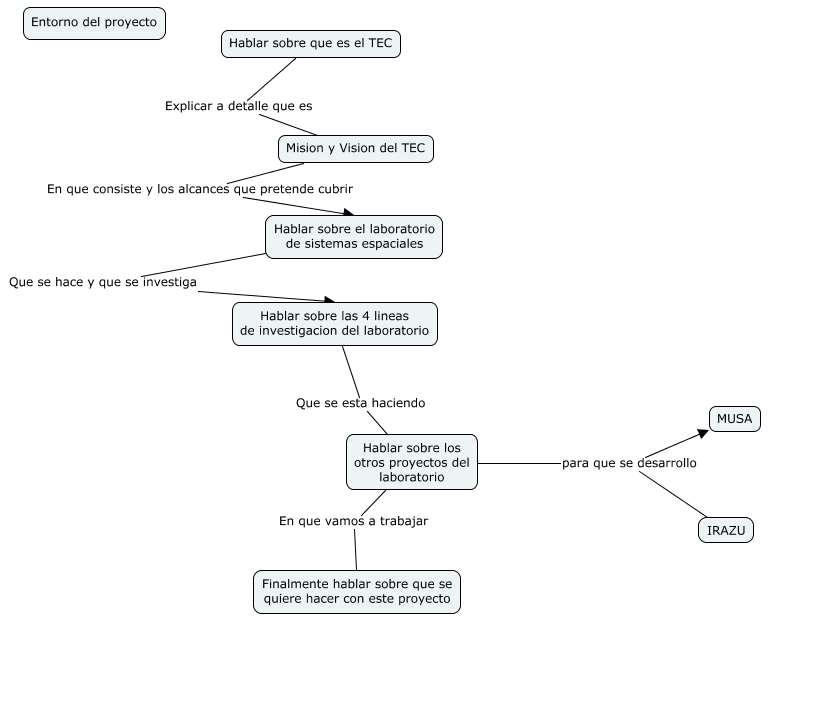
\includegraphics[width=0.8\textwidth]{Mapas conceptuales por seccion del anteproyecto/Diagrama_Entorno_del proyecto.png}
        \caption{Entorno del proyecto}
        \label{fig:Entorno}
      \end{figure}
      \newpage

      \begin{figure}[h!]
        \centering
        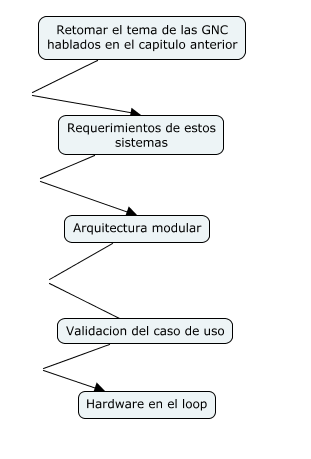
\includegraphics[width=0.3\textwidth]{Mapas conceptuales por seccion del anteproyecto/Diagrama_Entorno.png}
        \caption{Definicion del problema}
        \label{fig:definicion}
      \end{figure}


      \bf{Fecha de trabajo:} 8/08/2024.\\
      \bf{Objetivo:} Corrección de observaciones realizadas al anteproyecto.
      
      % Please add the following required packages to your document preamble:
      % \usepackage{graphicx}
      \begin{table}[h!]
          \label{tab:my-table}
          \resizebox{\textwidth}{!}{%
          \begin{tabular}{|l|}
          \hline
          \hline
          \multicolumn{1}{|c|}{Reporte de   actividades} \\ \hline
          \hline
          - Se aassssgrega el nombre del software propietario a utilizar a la Alternativa 1 : Matlab y Simulink.\\ \hline\hline
          \multicolumn{1}{|c|}{Productos obtenidos}                            \\ \hline\hline
          Se especifica para la Alternativa 1 el software a utilizar con el fin de delimitar la solucion a un marco de trabajo.\\ \hline
          \end{tabular}%
          }
          \end{table}
      

\end{document}